\newpage
\section{Mottakstank}
Mottakstanken er cirka 100 kubikkmeter og ligger som kjeller på anlegget. Vatnet blir lagra i mottaktstanken før det pumpast vidare til reaktorane. 
Mottakstanken fungerer også som utjamningstank og samlar varierande tilstrøymingar for å gi resten av anlegget homogene forhold.
Mottaktstanken har fire sensorar:
\begin{itemize}
    \item Trykkgivar for nivå (PP00-LT01) 
    \item Trykkgivar for overløp (PP00-LT02) 
    \item Flottør-vippe lav (PP00-LS02) 
    \item Flottør-vippe høg (PP00-LS01) 
\end{itemize}
Alle sensorane i mottaktstanken heng ifrå taket. Sensorane er tilgjengelege frå tilgangsluka som også er i taket på mottaktstanken.

Nivået i mottaktstanken blir primært målt med trykkgivar LT01 men kan også estimerast med flottør-vippene. For at vatnet skal pumpast vidare må trykkgivaren indikere at nivået er høgt nok. 
LS02 fungerer som backup.
I toppen av mottaktstanken er det ei open kasse. Denne kassa er delt i to med ein liten skiljevegg som er mindre enn høgda på kassa. I venstre kammer kjem reinsa vatn frå rektorane og renner vidare til resipient på sjølvfall (rein side). 
På høgre side ligger det ein trykkgivar som måler eventuelt overløp. Dersom nivået i mottaktstanken blir for høgt vil vatnet renne over til den opne kassa, 
aktivere trykkgivar, renne over skiljevegg og ut i resipient røyret som direkte overløp (skitten side). (Sjå illustrasjon)

Det er også overløpsrøyr tilbake til mottaktstanken frå reaktortankane samt ein retur av rejektvatn frå slamelamineringsanlegget sjå punkt xx.xx

\newpage
\begin{figure}[htbp]
    \centering
    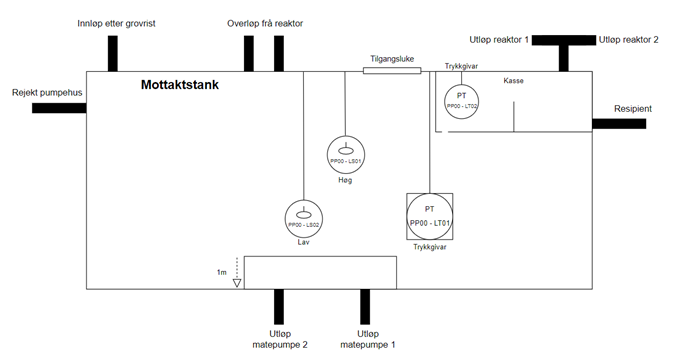
\includegraphics[width=1\textwidth]{Figurar/Mottakstank.png}
    \caption{Illustrasjon Mottakstank}\label{fig:Mottakstank}
\end{figure}

\begin{figure}[htbp]
    \centering
    \includegraphics[width=0.6\textwidth]{Figurar/utløpskasse.png}
    \caption{Illustrasjon utløpskasse}\label{fig:utløpskasse}
\end{figure}

